% This is where Assessors will be looking for signs of success and for evidence of thorough and systematic evaluation. Sample output, tables of timings and photographs of workstation screens, oscilloscope traces or circuit boards may be included. Care should be employed to take a professional approach throughout. For example, a graph that does not indicate confidence intervals will generally leave a professional scientist with a negative impression. As with code, voluminous examples of sample output are usually best left to appendices or omitted altogether.

% There are some obvious questions which this chapter will address. How many of the original goals were achieved? Were they proved to have been achieved? Did the program, hardware, or theory really work?

% Assessors are well aware that large programs will very likely include some residual bugs. It should always be possible to demonstrate that a program works in simple cases and it is instructive to demonstrate how close it is to working in a really ambitious case.

% graphs, performance, ablation
% run in mininet
% https://hub.docker.com/r/iwaseyusuke/mininet/
% discuss the implications of the graph
%base on evaluation chapter of papers!

\textit{In this section we highlight the methods and hardware used in evaluation [\ref{testingmethods}], benchmark the performance of Cap'n Proto and the Tezos cryptography library [\ref{librarybenchmarks}], and finally evaluate the performance of our HotStuff implementation [\ref{hotstuffbenchmarks}]}

\section{Testing methodology} \label{testingmethods}
% describe sofia server
Evaluation was carried out on the computer laboratory's Sofia server (2x Xeon Gold 6230R chips, 768GB RAM). Carrying out experiments on the server should help to minimise interference from other processes on the system.

Experiments were driven by an open-loop load generator (see \ref{loadgenerator}), and were automated using Python scripts (see \ref{experimentscripts}). In all experiments the load generator was run for 10 seconds, with a further 10 seconds after this without the load generator running to wait for any slow responses.

\section{Library benchmarks} \label{librarybenchmarks}
\subsection{Cap'n Proto} \label{capnpbenchmark}

\begin{figure}[h!]
\centering
\includegraphics[scale=0.75]{dummy_test/throughputgoodput.png}
\caption{Benchmarking of Cap'n Proto server goodput for varying throughputs and message sizes, run for 10s}
\end{figure}

\begin{figure}[h!]
\centering
\includegraphics[scale=0.75]{dummy_test/throughputflatency.png}
\caption{Benchmarking of Cap'n Proto server latencies for varying throughputs and message sizes, run for 10s. Discarded result if goodput was not within 5\% of target throughput.}
\end{figure}

\begin{figure}[h!]
\centering
\includegraphics[scale=0.75]{dummy_test/throughputlost.png}
\caption{Benchmarking of Cap'n Proto server \% of failed requests for varying throughputs and message sizes, run for 10s}
\end{figure}

[describe the experiment methodology, present argument, then back up with evidence from figures]
We benchmarked the latency and goodput of sending messages in Cap'n Proto. We varied the size of messages sent in different tests to replicate the behaviour of the algorithm when sending `batches' of many commands, so a message size of 600 means that the message size is approximately that of a message containing 600 commands.

The figures demonstrate that the framework has a severe drop in performance when sending large messages. For a message size of 600 the goodput goes to zero as the throughput increases, meaning that no messages are being responded to.

[``Fundamentally, there are limitations in the RPC framework that give an upper bound on the performance we can hope to achieve, these limitations are evident in our benchmarking of the Cap'n Proto framework\dots'']

\subsection{Tezos Cryptography} \label{tezosbenchmark}
I profiled the important functions of the library with Jane Street's Core\_bench module [citation needed***]. Core\_bench is a micro-benchmarking library used to estimate the cost of operations in OCaml, it runs the operation many times and uses linear regression to try to reduce the effect of high variance between runs.

\begin{table}[!h]
	\centering
	\begin{tabular}{|l|r|}
	\hline
	Function                 & Time (µs) \\ \hline
	Sign                     & 427.87   \\
	Check                    & 1,171.77 \\
	Aggregate (4 sigs)       & 302.90   \\
	Aggregate check (4 sigs) & 1,179.25 \\
	Aggregate (8 sigs)       & 605.38   \\
	Aggregate check (8 sigs) & 1,180.61 \\ \hline
	\end{tabular}
	\caption{Benchmarking of key functions of the Tezos Cryptography library}
\end{table}
% ┌─────────────┬────────────┬─────────┬──────────┬──────────┬────────────┐
% │ Name        │   Time/Run │ mWd/Run │ mjWd/Run │ Prom/Run │ Percentage │
% ├─────────────┼────────────┼─────────┼──────────┼──────────┼────────────┤
% │ sign        │   427.87us │ 144.00w │          │          │     36.24  │
% │ check       │ 1_171.77us │  75.00w │          │          │     99.25  │
% │ agg_4       │   302.90us │ 484.00w │    0.15w │    0.15w │     25.66  │
% │ agg_check_4 │ 1_179.25us │  75.00w │          │          │     99.88  │
% │ agg_8       │   605.38us │ 944.00w │    0.35w │    0.35w │     51.28  │
% │ agg_check_8 │ 1_180.61us │  75.00w │          │          │    100.00  │
% └─────────────┴────────────┴─────────┴──────────┴──────────┴────────────┘

\section{HotStuff implementation benchmarks} \label{hotstuffbenchmarks}
Our implementation achieves a reasonable level of performance due to the optimisations described in section \ref{performance}, but is fundamentally limited in what it can achieve due to constraints on bandwidth from the Cap'n Proto library (see \ref{capnpbenchmark}), and on latency from the Tezos cryptography library (see \ref{tezosbenchmark}).

We demonstrate the effectiveness of our performance improvements in an ablation study in section \ref{ablation}. There is further evidence for the effectiveness of batching (see section \ref{batching}); the system is able to achieve much higher goodputs with batch sizes greater than one (equivalent to not batching at all), as shown in section \ref{batchsizeseval}. 

The constraints on bandwidth from using Cap'n Proto are evident in our comparisons of batch sizes (see section \ref{batchsizeseval}), and of node counts (see section \ref{nodecountseval}). The goodput that can be achieved increases with batch size before reaching a maximum and declining, as Cap'n Proto is unable to handle the higher bandwidth caused by larger batches. Increasing the node count increases the number of internal messages, so system performance declines for higher node counts, again due to poor message sending performance.

The latency cost of Tezos cryptography is clear from the superior performance of the system with cryptography disabled, as shown in the ablation study (see section \ref{ablation}).
% The system maintains a stable bound on latency up to a certain throughput [reference heatmap with stable latency], but experiences exponential growth in latency when it can no longer keep up with the volume of requests [reference heatmap with exponential latency]. This exponential growth is due to queues of requests building on each node; as the test progresses the length of the queues increases linearly, causing the wait time to grow exponentially??? throughput/latency?
\subsection{Batch sizes} \label{batchsizeseval}
blah blah batch sizes

\begin{figure}[h!]
\centering
\includegraphics[scale=0.75]{batch_size_test/throughputgoodput.png}
\caption{Benchmarking of goodput for varying throughputs and batch sizes, run for 10s}
\end{figure}

\begin{figure}[h!]
\centering
\includegraphics[scale=0.75]{batch_size_test/throughputflatency.png}
\caption{Benchmarking of mean latency while varying throughputs and batch sizes, run for 10s. Discarded result if goodput was not within 5\% of target throughput.}
\end{figure}

\begin{figure}[h!]
\centering
\includegraphics[scale=0.75]{batch_size_test/throughputlost.png}
\caption{Benchmarking of \% requests lost while varying throughputs and batch sizes, run for 10s.}
\end{figure}

\begin{figure}[h!]
\centering
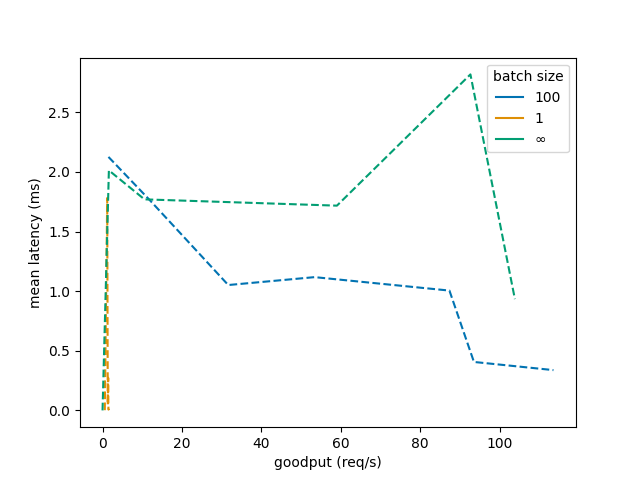
\includegraphics[scale=0.75]{mininet/throughputlatency.png}
\caption{Benchmarking of mean latency while varying throughputs and batch sizes, run for 10s with 100ms network delay.}
\end{figure}

\begin{figure}[h!]
\centering
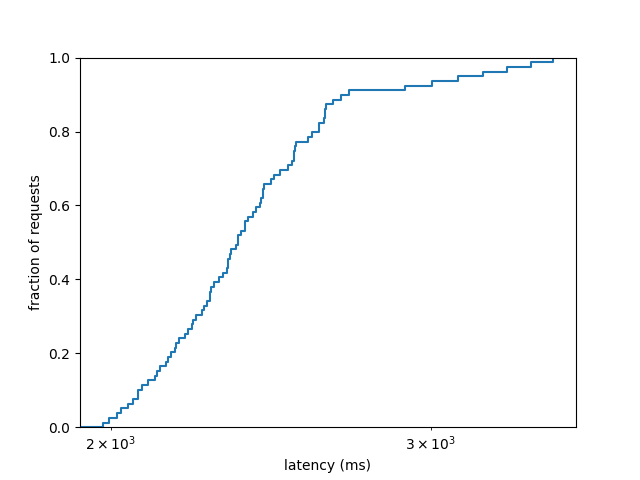
\includegraphics[scale=0.75]{mininet/10tpub_cumlatency.png}
\caption{Cumulative latency plot for experiment with a throughput of 10req/s and unlimited batch size, run for 10s with 100ms network delay.}
\end{figure}

\subsection{Node counts} \label{nodecountseval}
blah blah node counts

\begin{figure}[h!]
\centering
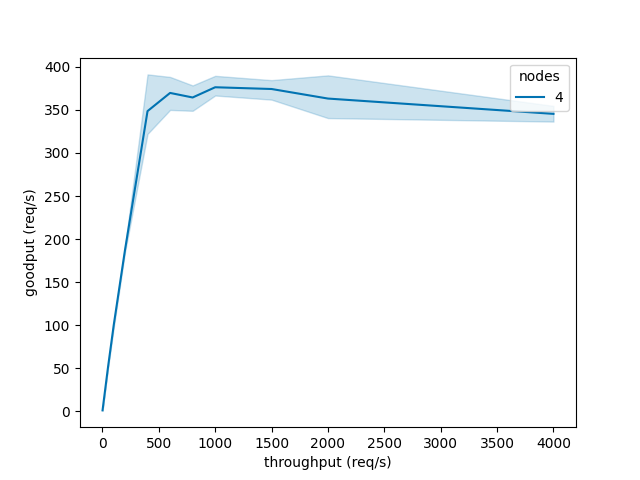
\includegraphics[scale=0.75]{node_count_test/throughputgoodput_nodes.png}
\caption{Benchmarking of goodput for varying throughputs and node counts, run for 10s}
\end{figure}

\begin{figure}[h!]
\centering
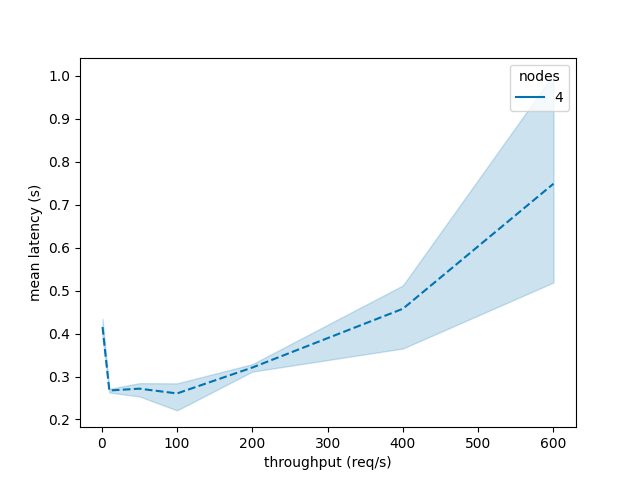
\includegraphics[scale=0.75]{node_count_test/throughputflatency_nodes.png}
\caption{Benchmarking of mean latency while varying throughputs and node counts, run for 10s. Discarded result if goodput was not within 5\% of target throughput.}
\end{figure}

\begin{figure}[h!]
\centering
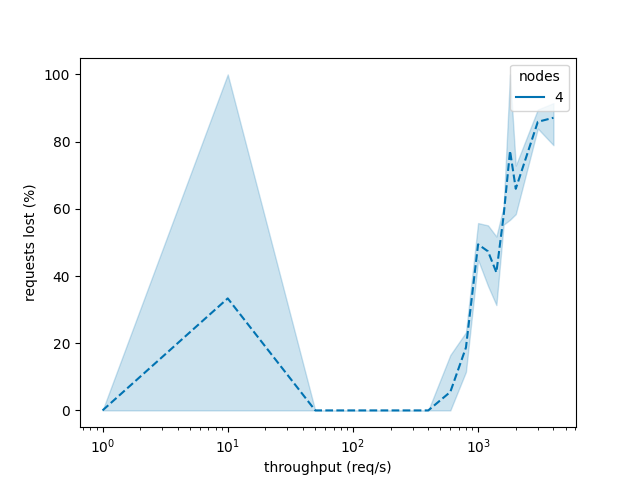
\includegraphics[scale=0.75]{node_count_test/throughputlost_nodes.png}
\caption{Benchmarking of \% requests lost while varying throughputs and node counts, run for 10s.}
\end{figure}

\subsection{Ablation study} \label{ablation}
[``This change (changing the pull function) improved performance by reducing the amount of time spent waiting in the main loop, the difference is shown in an ablation study'']
blah blah ablation.
[run with crypto disabled for comparison]

Versions:
[turn me into a table!! with caption ``versions'']
\begin{enumerate}
	\item Unchained version
	\item Chained version - node truncation disabled, command filtering disabled
	\item Chained version - node truncation disabled, command filtering enabled
	\item Chained version - node truncation enabled, command filtering disabled
	\item Chained version - node truncation enabled, command filtering enabled
\end{enumerate}

\begin{figure}[h!]
\centering
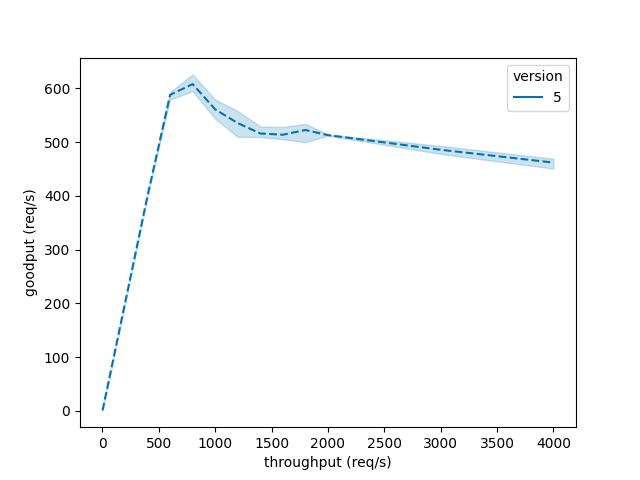
\includegraphics[scale=0.75]{ablation/throughputgoodput_ablation.png}
\caption{Benchmarking of goodput for varying throughputs and implementation versions, run for 10s with 4 nodes unlimited batch size.}
\end{figure}

\begin{figure}[h!]
\centering
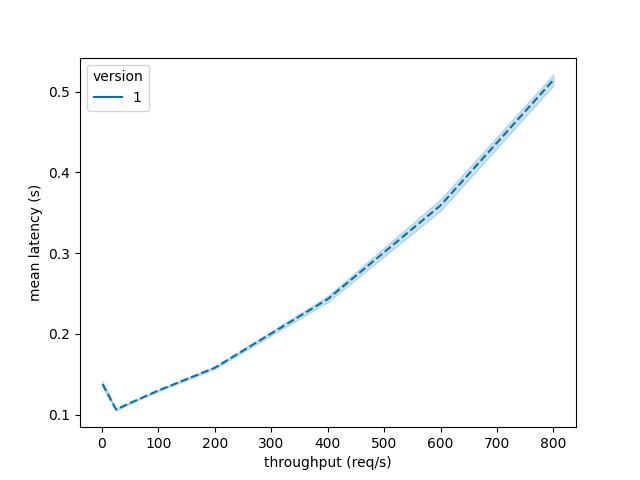
\includegraphics[scale=0.75]{ablation/throughputflatency_ablation.png}
\caption{Benchmarking of mean latency while varying throughputs and implementation versions, run for 10s with 4 nodes unlimited batch size. Discarded result if goodput was not within 5\% of target throughput.}
\end{figure}

\begin{figure}[h!]
\centering
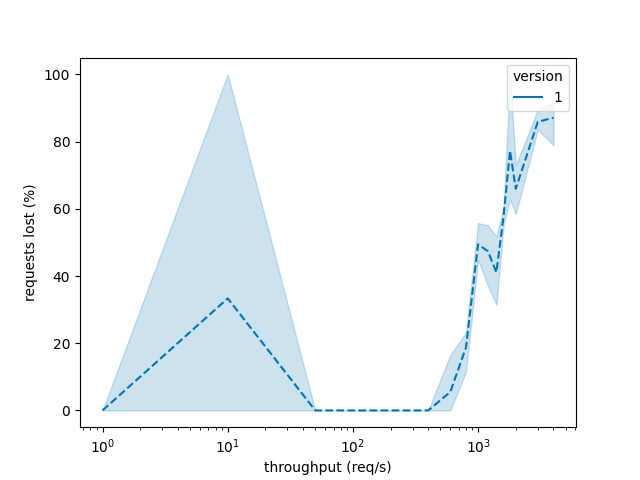
\includegraphics[scale=0.75]{ablation/throughputlost_ablation.png}
\caption{Benchmarking of \% requests lost while varying throughputs and implementation versions, run for 10s with 4 nodes unlimited batch size.}
\end{figure}

\subsection{View change}
\begin{figure}[h!]
\centering
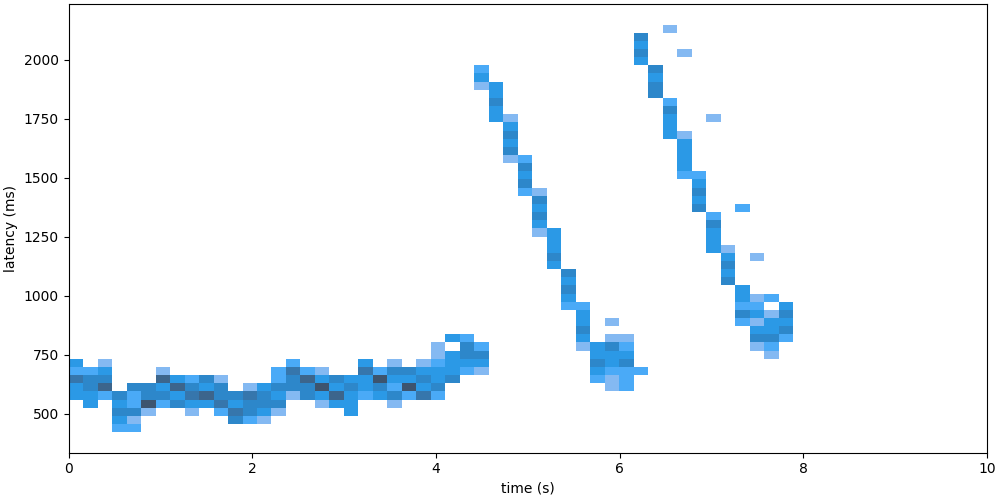
\includegraphics[scale=0.5]{viewchange/test7_100_7_100_timelatencyheatmap.png}
\caption{Heatmap showing distribution of latencies with a node being killed 5s in. Run for 10s with 7 nodes and a batch size of 100.}
\end{figure}
% Clone github.com/cjen1/reckon

% ```
% # This is likely to take a while
% make reckon-mininet

% docker run -it --privileged -e DISPLAY --network host --name reckon-mininet cjen1/reckon:latest bash

% # Set up mininet net with a single switch and 3 nodes
% # drops you into a cli (you can also use python scripting)
% mn --topo single,3

% # observe no delay between nodes
% mininet> h1 ping h2
% mininet> <Ctrl-C>/<Ctrl-D> to exit

% # syntax is `mininet> <node> <command>`
% # I run screens on each node and then attach to those from outside mininet to run the tests in different terminal screens. (Tmux doesn't work correctly afaicr)

% mininet> h1 screen -dmS node_h1 bash

% #Then in another terminal session
% docker exec -it reckon-mininet bash
% screen -r node_h1
% <whatever commands you want to run on that emulated node>

% #Similarly for the other nodes
% ```